\documentclass{article}

\usepackage[utf8]{inputenc}

\usepackage{natbib}

\usepackage{bookmark}

\usepackage[italian]{babel}

\usepackage{graphicx}
\graphicspath{ {./images/} }

\usepackage{float}

\usepackage{soul}


\usepackage{listings}
\usepackage{color}
\definecolor{lightgray}{rgb}{.97,.97,.97}
\definecolor{darkgray}{rgb}{.4,.4,.4}
\definecolor{purple}{rgb}{0.65, 0.12, 0.82}
\lstdefinelanguage{JavaScript}{
	keywords={exports, require, typeof, new, true, false, catch, function, return, null, catch, switch, var, const, if, in, while, do, else, case, break},
	keywordstyle=\color{blue}\bfseries,
	ndkeywords={class, export, boolean, throw, implements, import, this},
	ndkeywordstyle=\color{darkgray}\bfseries,
	identifierstyle=\color{black},
	sensitive=false,
	comment=[l]{//},
	morecomment=[s]{/*}{*/},
	commentstyle=\color{purple}\ttfamily,
	stringstyle=\color{red}\ttfamily,
	morestring=[b]',
	morestring=[b]"
}
\lstset{
	language=JavaScript,
	backgroundcolor=\color{lightgray},
	extendedchars=true,
	basicstyle=\footnotesize\ttfamily,
	showstringspaces=false,
	showspaces=false,
	numbers=left,
	numberstyle=\footnotesize,
	numbersep=9pt,
	tabsize=2,
	breaklines=true,
	showtabs=false,
	captionpos=b
}


\newcommand{\paragraphNewline}{\\[0.2cm]}
\newcommand{\removeHorizontalSpaceSmall}{\hspace{-0.36cm}}
\newcommand{\removeHorizontalSpaceBig}{\hspace{-0.525cm}}


\begin{document}

\title{
    Nim Multiplayer \\
    \large Applicazioni e Servizi Web
}

\author{Bondi Davide - 0000885217 \{davide.bondi3@studio.unibo.it\}}

\date{11 Ottobre 2021}

\maketitle
\newpage

\section{Introduzione}

Nim Multiplayer è un'applicazione web che permette a 2 o più utenti di giocare a Nim (\href{https://it.wikipedia.org/wiki/Nim}{https://it.wikipedia.org/wiki/Nim}). Nim è un gioco matematico che coinvolge 2 giocatori. Nim Multiplayer supporta le partite 1 vs 1, ed aggiunge regole per gestire le partite multi giocatore.

\begin{figure}[h]
	\centering
	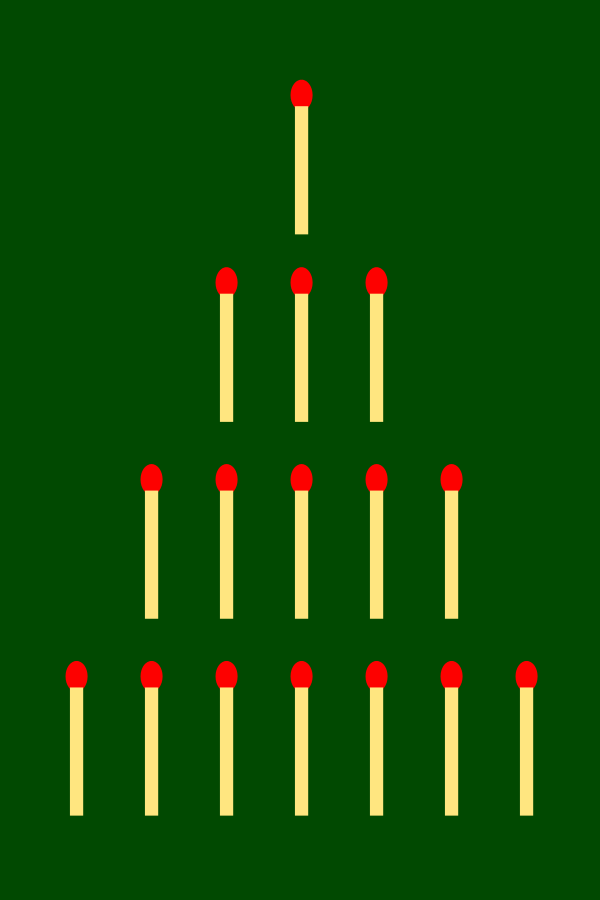
\includegraphics
	[width=0.25\linewidth]
	{wikipedia - 600px-NimGame.svg}
	\caption{una partita Nim\cite{nim_wikipedia}.}
	%\label{fig:nim-logo}
\end{figure}

Per giocare a Nim, i 2 giocatori, a turno, rimuovono gli "\emph{oggetti} o \emph{elementi}" da "\emph{cumuli} o \emph{pile}" distinti.

Per maggiore chiarezza, in questo progetto si è scelto di utilizzare termini più specifici (e ritenuti più appropriati) per esprimere il gergo del gioco: gli "\emph{oggetti} o \emph{elementi}", data la loro forma, assumono il nome di \emph{bastoncini}; mentre i "\emph{cumuli} o \emph{pile}" vengono definiti semplicemente come \emph{righe} o \emph{righe di bastoncini}.

Durante il proprio turno, la mossa consiste nel rimuovere un numero qualsiasi di bastoncini posti su una qualsiasi e unica riga, ma tali bastoncini devono essere adiacenti e tra loro non vi devono essere altri bastoncini già rimossi (non è possibile saltare la mossa nel proprio turno).

A seconda della versione, l'obiettivo del gioco è evitare di rimuovere l'ultimo bastoncino (versione \emph{Marienbad} o \emph{misère}) o rimuovere l'ultimo bastoncino (versione \emph{standard}).

Il numero di bastoncini e di righe sono concordati a piacere tra i giocatori all'inizio della partita.

Il Nim è divenuto piuttosto famoso perché ha una strategia di vittoria semplice (ha classe di complessità L), facilmente utilizzabile come esempio in teoria dei giochi, in particolare questa si basa sul calcolo binario\cite{nim_wikipedia}.

In breve, Nim Multiplayer modella: il gioco Nim tradizionale con vittoria \emph{standard} e \emph{Marienbad}; aggiunge una variante riguardo la rotazione dei turni (turni chaos); aggiunge regole per la gestione della vittoria \emph{standard} e \emph{Marienbad} in partite multi giocatore.

\newpage

\section{Requisiti}

\subsection{Funzionali}
\label{requisiti funzionali}

\begin{itemize}
\item
	Registrazione di un nuovo utente e servizio di login.
\item
	Creazione di una stanza di gioco e relativi inviti.
\item
	Configurare le opzioni di gioco, durante la creazione di una nuova partita.
	\begin{itemize}
	\item
		Scegliere il numero di giocatori.
	\item
		Scegliere il numero di righe di bastoncini.
	\item
		Scegliere la rotazione dei turni: rotazione oppure chaos.
	\item
		Scegliere la modalità di vittoria: Standard oppure Marienbad.
	\end{itemize}
\item
	Gestione di una partita Nim tradizionale (1 vs 1): svolgimento del turno; rotazione dei turni (2 tipologie); modalità di vittoria (2 tipologie).
	\begin{itemize}
	\item
		Svolgimento del turno: durante il proprio turno, la mossa consiste nel rimuovere un numero qualsiasi di bastoncini posti su una qualsiasi e unica riga, ma tali bastoncini devono essere adiacenti e tra loro non vi devono essere altri bastoncini già rimossi (non è possibile saltare la mossa nel proprio turno).
	\item
		Rotazione dei turni (2 tipologie).
		\begin{itemize}
		\item
			La tipica rotazione: i giocatori si alternano in un ordine prestabilito per tutta la durata della partita, generato casualmente ad inizio partita.
		\item
			Turni \emph{chaos}: il gioco procede a turni casuali, ovvero il gioco sceglierà di far passare il turno casualmente ad un giocatore fra quelli che sono "indietro di un turno".
		\end{itemize}
	\item
		Modalità di vittoria (2 tipologie).
		\begin{itemize}
		\item
			Standard: il giocatore che rimuove l'ultimo bastoncino vince.
		\item
			Marienbad: il giocatore che rimuove l'ultimo bastoncino perde.
		\end{itemize}
	\end{itemize}
\item
	Gestione di una partita multiplayer (fino a 6 giocatori).
	\begin{itemize}
	\item
		Svolgimento del turno e rotazione dei turni: sono identici ai concetti descritti nei punti precedenti.
	\item
		Modalità di vittoria (2 tipologie).
		\begin{itemize}
		\item
			Standard: identica a 1 vs 1 (il giocatore che rimuove l'ultimo bastoncino vince, e la partita finisce).
		\item
			Marienbad: il giocatore che rimuove l'ultimo bastoncino viene eliminato dalla partita, ed il gioco prosegue nel seguente modo finché non rimarrà un solo giocatore (vincitore). Dopo l'eliminazione di un giocatore, i bastoncini nelle righe vengono tutti ripristinati, ad eccezione dei bastoncini rimossi dai giocatori eliminati.
		\end{itemize}
	
	\newpage
	
	\item
		Gestione delle disconnessioni dei giocatori. Le disconnessioni vengono gestite quando si presenta il turno del giocatore disconnesso.
		\begin{itemize}
		\item
			Vittoria Standard: quando si verifica la disconnessione di un giocatore, quest'ultimo viene eliminato dalla partita senza alterare i bastoncini in gioco.
		\item
			Vittoria Marienbad: la disconnessione di un giocatore è considerata come una eliminazione, per cui verranno ripristinati i bastoncini opportuni.
		\end{itemize}
	\end{itemize}
\end{itemize}

\subsection{Non Funzionali}

\begin{itemize}
\item
	Connessione sicura tramite https (implementato).
\item
	Memorizzazione cifrata delle password nel database (implementato).
\item
	Recupero delle credenziali utente, tramite invio di una mail (non implementato).
\item
	Giocare una partita come guest non registrato (non implementato).
\item
	Osservare una partita (non implementato).
\item
	Aggiungere nel server un task dedicato per identificare periodicamente le partite finite e le partite mai iniziate, per poi cancellarle e ridurre ragionevolmente lo spazio di archiviazione del database (non implementato).
\end{itemize}

\subsection{Requisiti Tecnologici}

L'applicazione verrà realizzata con il solution stack MEVN.

Le comunicazioni real time riguardo la creazione e la gestione della stanza di gioco verranno implementate con la libreria Socket.IO.

\subsection{Requisiti degli Utenti}

Il metodo di design scelto è \emph{user centered design} (UCD), il quale pone il focus sui bisogni degli utenti in modo iterativo, al fine di massimizzare il grado di soddisfazione della \emph{user experience} (UX).

Per questo è stata svolta un'analisi dei \emph{target user}, e sono state simulate alcune \emph{Personas} come modelli "virtuali" di utenti, correlate ad uno \emph{scenario d'uso} specifico. Ecco la lista di \emph{Personas} considerate.

\begin{itemize}
\item
	Simone conosce la versione tradizionale di Nim e conosce il "segreto" celato dietro la "complessità" del gioco.
	\newline
	Simone gioca partite 1 vs 1, con modalità di vittoria standard, e turni svolti rigorosamente in rotazione.
\item
	Eraldo ha giocato sempre e solo la versione tradizionale di Nim con modalità di vittoria Marienbad. Ripudia la vittoria standard perché secondo lui non è la versione originale, pertanto non deve essere giocata.
	\newline
	Eraldo gioca partite 1 vs 1, con modalità di vittoria Marienbad, e turni svolti in rotazione.
\item
	Ilaria è completamente estranea a giochi matematici e combinatori, tuttavia vorrebbe comunque essere partecipe e giocare insieme ai suoi amici. Talvolta vorrebbe anche poter vincere senza necessariamente dover capire la classe di complessità del gioco.
	\newline
	Ilaria gioca partite multiplayer con gli amici, con qualsiasi modalità di vittoria, e turni svolti in modalità chaos.
\item
	Lorenzo è il classico nerd che conosce a fondo i giochi matematici e giochi strategici che includono il calcolo combinatorio, a volte si cimenta in tornei di scacchi piuttosto impegnativi. Per lui il Nim è un gioco estremamente semplice e noioso.
	\newline
	Lorenzo gioca partite multiplayer con il numero massimo di giocatori consentito, con modalità di vittoria Marienbad (perché le partite sono più lunghe e richiedono un piccolo sforzo mnemonico), e turni svolti rigorosamente in rotazione.
\end{itemize}

\newpage

\section{Design}

\subsection{Design delle Interfacce Utente}
\label{design delle interfacce utente}

In questa sezione si conclude l'analisi della \emph{Human Computer Interaction} (HCI), iniziata durante l'identificazione delle Personas precedenti.

Nelle applicazioni web è consono seguire un approccio di design \emph{mobile first} per progettare le interfacce utente, e così è stato fatto. In particolare, il \emph{progressive enhancement} dell'applicazione si è fermato proprio a livello mobile, cioè non sono stati aggiunti ulteriori raffinamenti significativi per i dispositivi desktop, poiché l'applicazione ed il gioco in sè, sono due elementi talmente minimali, in cui tutto quello da disporre nell'interfaccia è esposto in maniera ottimale anche nei dispositivi mobile.

Questo fattore non esclude il fatto che l'applicazione dispone di \emph{responsive design} e \emph{layout liquido}, ovvero, nonostante l'interfaccia dell'applicazione risulta praticamente identica in tutti i dispositivi, in realtà essa è più fruibile e più "confortevole" nei dispositivi desktop, in quanto gli elementi dell'interfaccia sono disposti su un viewport più largo e si adattano ad esso, migliorando la \emph{user experience} e l'\emph{usabilità} dell'applicazione. Un esempio: nei dispositivi mobile per leggere le regole del gioco bisogna scrollare a fondo, mentre nei dispositivi desktop è sufficiente scrollare meno. Un altro esempio: nei dispositivi desktop, i bastoncini sono renderizzati con una qualità di immagine migliore.

Qui di seguito sono rappresentati i \emph{mockup} prodotti durante la fase di design delle interfacce utente. Per contestualizzarli in relazione all'\emph{usabilità} dell'applicazione, sono stati raggruppati in due principali \emph{storyboard}.

I \emph{mockup} sono stati realizzati tramite Pencil, il quale dispone di feature per creare mockup interattivi (inter-page linking\cite{pencil_website}), ma non dispone di feature per creare \emph{storyboard}, per cui quelle inserite qui di seguito sono state prodotte con un editor generico per immagini.

La \emph{storyboard} in figura \ref{fig:storyboard - user session} rappresenta l'insieme di task inerenti alla gestione dei dati dell'utente. Mentre la \emph{stroryboard} in figura \ref{fig:storyboard - game task} rappresenta il task che svolge un utente per creare e giocare una partita.

Un approccio piuttosto informale, ma allo stesso tempo molto pratico per valutare l'\emph{usabilità} del design delle interfacce, consiste nell'osservare l'applicazione nell'ottica delle \emph{euristiche di Nielsen}. Svolgendo questa analisi, si ritiene che tutte le euristiche siano pienamente soddisfatte, soprattutto grazie al fatto della semplicità del sistema modellato.

Osservando le due \emph{storyboard} in figura \ref{fig:storyboard - user session} e \ref{fig:storyboard - game task}, si intuisce che le rotte dell'applicazione appartengono a due categorie principali: al dominio dei dati utente, oppure al dominio di gioco. Queste due categorie sono molto importanti, perché sono state sfruttate per modularizzare il design e il codice in molteplici punti.

\newpage

\begin{figure}[H]
	\centering
	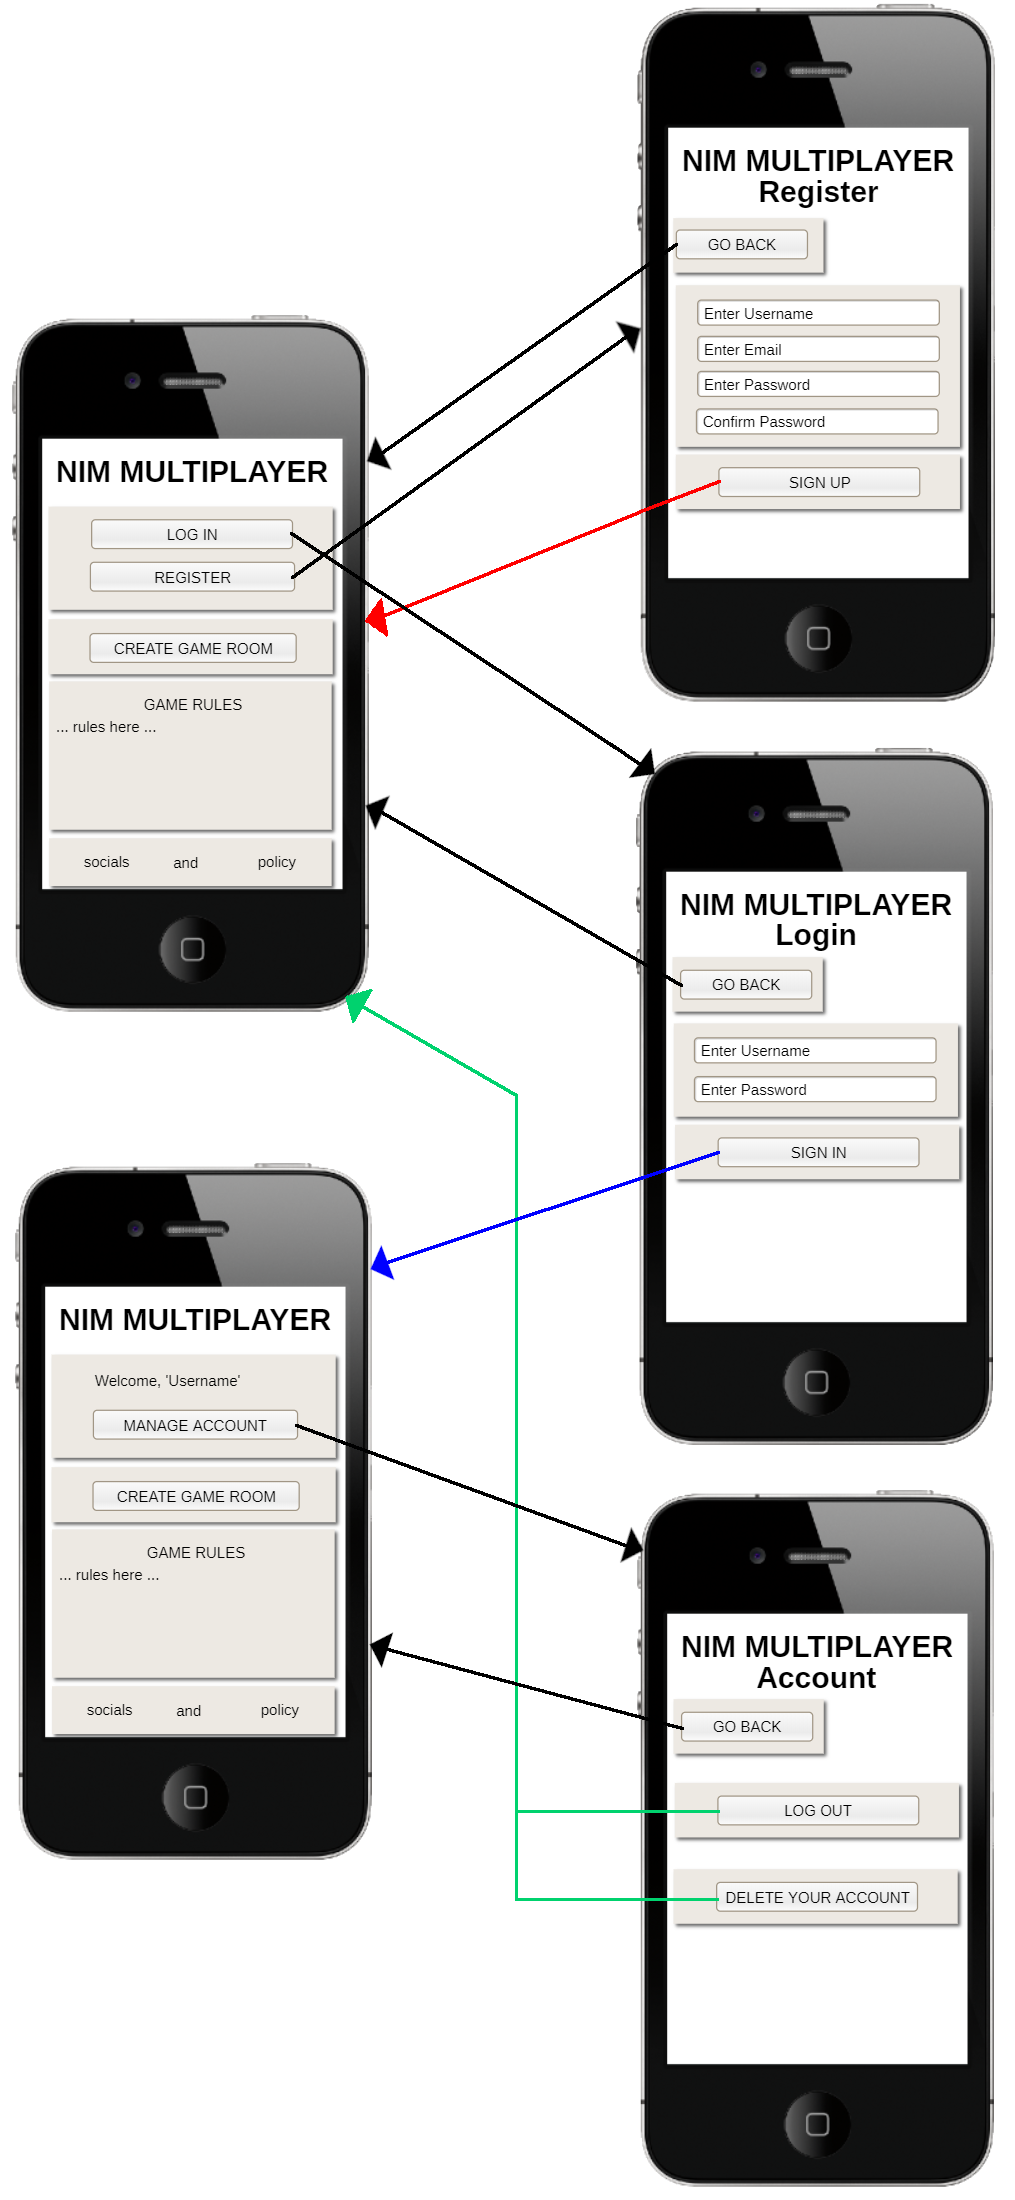
\includegraphics
	[width=0.65\linewidth]
	{storyboard with mockup - user session}
	\caption{storyboard con i mockup per gestire il dominio dei dati utente.
		\newline
		Linee nere: navigazione che non causa alcuna modifica al sistema.
		\newline
		Linea rossa: registrazione di un nuovo account utente.
		\newline
		Linea blu: login di un utente.
		\newline
		Linee verdi: logout e/o eliminazione dell'account.
	}
	\label{fig:storyboard - user session}
\end{figure}

\newpage

\begin{figure}[H]
	\centering
	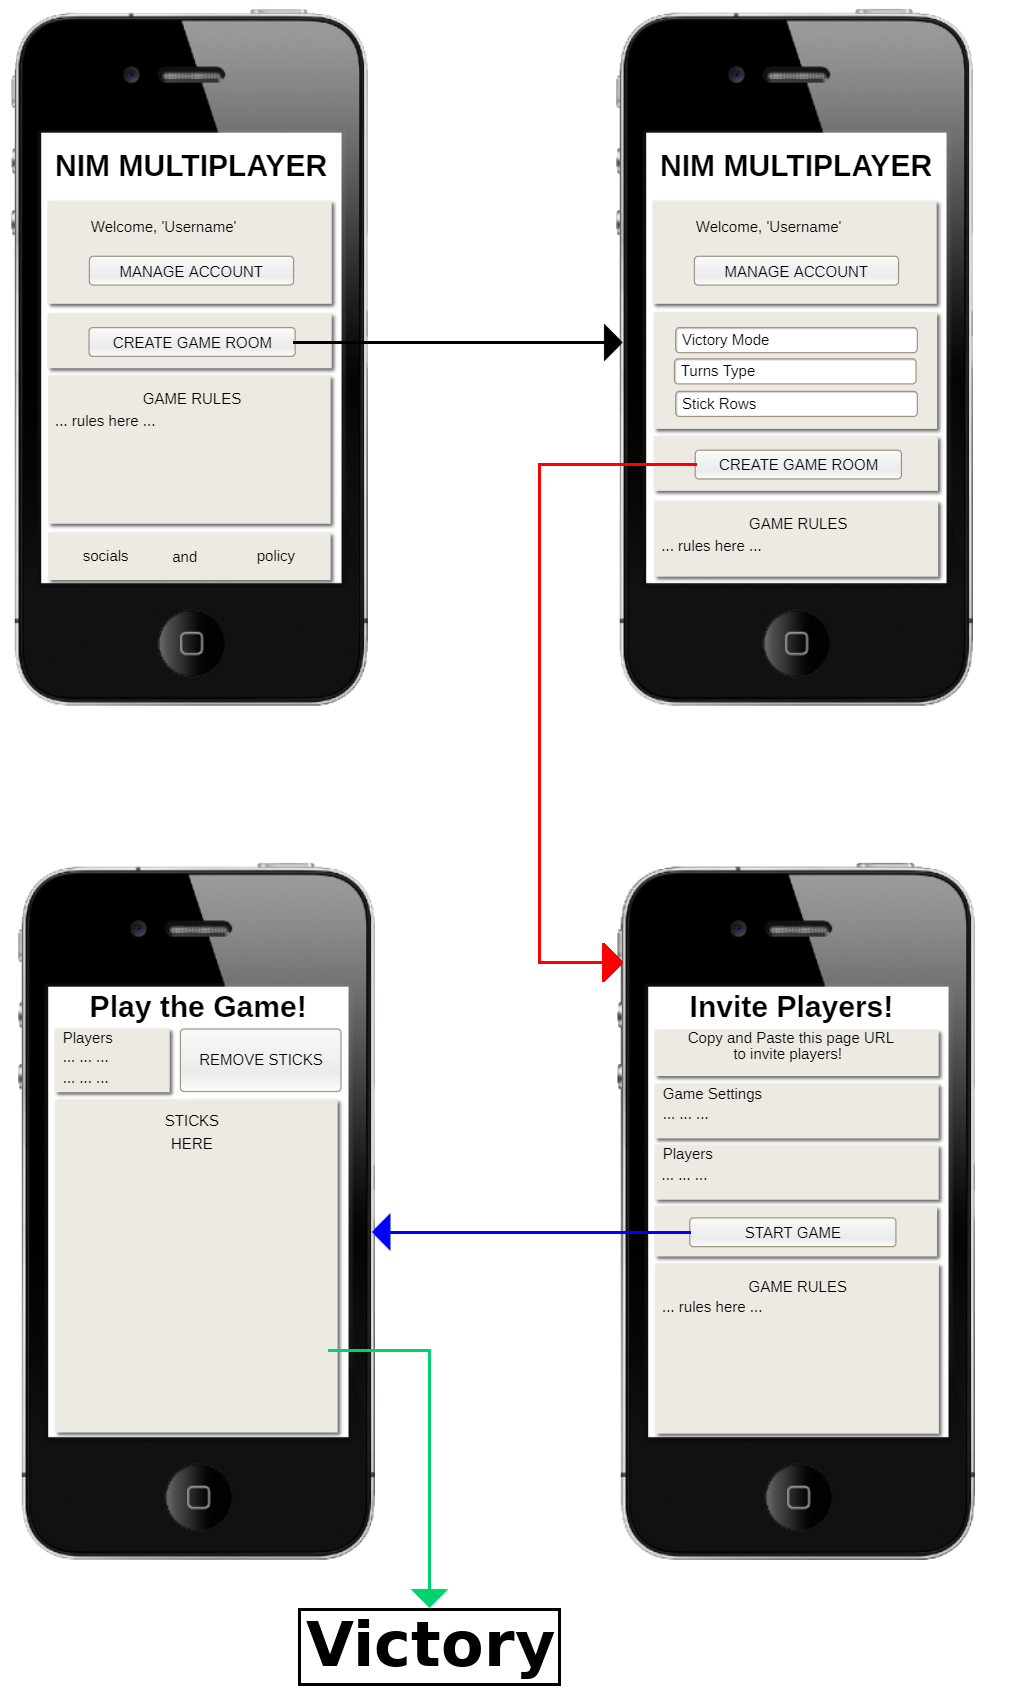
\includegraphics
	[width=0.66\linewidth]
	{storyboard with mockup - play the game}
	\caption{storyboard con i mockup per gestire la creazione e lo svolgimento di una partita (dominio di gioco).
		\newline
		Linea nera: navigazione che non causa alcuna modifica al sistema.
		\newline
		Linea rossa: creazione di una partita.
		\newline
		Linea blu: dopo aver invitato i giocatori desiderati, la partita comincia.
		\newline
		Linea verde: dopo aver giocato la partita, i giocatori sono indirizzati verso la pagina che indica il vincitore.
	}
	\label{fig:storyboard - game task}
\end{figure}

\newpage

Nella figura \ref{fig:storyboard - game task} si può osservare che il numero di giocatori non deve essere specificato prima di creare una nuova partita, bensì viene dedotto automaticamente in base a quanti utenti visitano la pagina della stanza di gioco. In questo modo, l'utente non deve scegliere il numero di giocatori, ma deve solo copiare l'URL della stanza di gioco ed inviarlo ai giocatori. Naturalmente, nella fase in cui vengono invitati i giocatori, in pagina deve essere riportato il numero massimo di giocatori che possono essere contenuti in una stanza di gioco.

\subsection{Design dell'Architettura di Sistema}

Il sistema da realizzare non richiede la gestione di situazioni particolarmente vincolanti, per questo si è scelto di adottare una soluzione di tipo \emph{Single Page Application} (SPA), al fine di ottimizzare la reattività dell'applicazione.

Di conseguenza, il layer della struttura HTML e il layer di presentazione CSS (quindi tutto ciò che riguarda la view di sistema) sono collocati totalmente a client side, mentre invece il layer di \emph{application logic} (o \emph{business logic}) è distribuito tra client e server.

\subsubsection{Front-end}
\label{design architettura - front-end}

Cercando di astrarre quanto più possibile dalle tecnologie utilizzate, la struttura della SPA deve essere organizzata nel seguente modo.

\begin{figure}[H]
	\advance\leftskip-1.2cm
	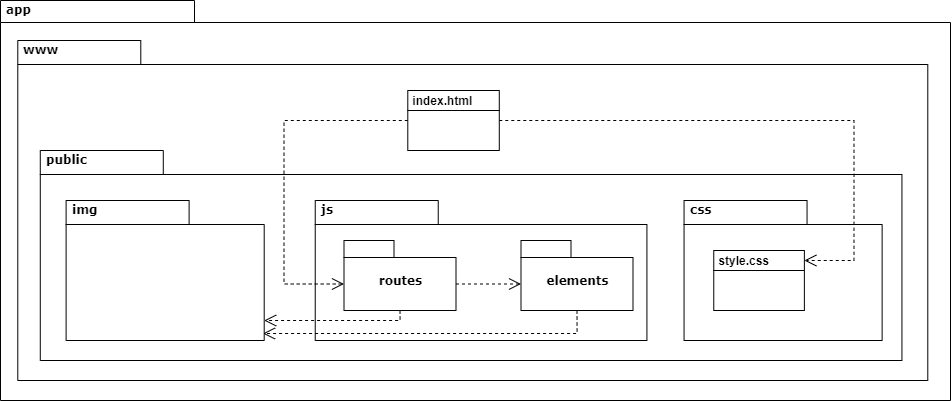
\includegraphics
	[width=1.2\linewidth]
	{package diagram - SPA}
	\caption{package diagram della SPA (la view situata a client side).
		\newline
		Per applicare maggiore chiarezza, il formalismo del package diagram è stato violato e sono stati inseriti i due file \texttt{index.html} e \texttt{style.css}, ma concettualmente il diagramma rappresenta comunque l'organizzazione e la dipendenza dei package e dei due file rappresentati.}
	\label{fig: package diagram - SPA}
\end{figure}

\newpage

\begin{enumerate}
\item
	Il file \texttt{index.html} è la \emph{Single Page}, la quale contiene al suo interno tutti gli import e la logica di \emph{Application}, quindi contiene tutti i framework o librerie e i file utilizzati a client side.
\item
	Il package \texttt{public} contiene tutti gli elementi importati ed utilizzati in \texttt{index.html}. Quindi \texttt{public} contiene l'implementazione dell'applicazione client side, e deve essere strutturato in questo modo.
	\begin{itemize}
	\item
		Il package \texttt{img} contiene le immagini.
	\item
		Il package \texttt{js} (Javascript) contiene gli elementi del framework che implementa la SPA, e deve avere a sua volta 2 sub-package.
		\begin{enumerate}
		\item
			Il package \texttt{routes} che contiene gli elementi che rappresentano le rotte (pagine) dell'applicazione.
		\item
			Il package \texttt{elements} che contiene gli elementi che rappresentano porzioni di HTML incapsulate e riutilizzate fra le rotte.
		\end{enumerate}
	\item
		Il package \texttt{css} contiene solo il file \texttt{style.css}, che rappresenta il layer di presentazione da importare in \texttt{index.html}.
	\end{itemize}
\end{enumerate}

Considerando ciò che è emerso dalla sezione \ref{design delle interfacce utente}, il package \texttt{public/js/routes} deve avere due sub-package per racchiudere i due domini presenti nel sistema: \texttt{routes/user} contiene le rotte del dominio dei dati utente; \texttt{routes/game} contiene le rotte del dominio di gioco.

\newpage

\subsubsection{Back-end}

Cercando di astrarre quanto più possibile dalle tecnologie utilizzate, la struttura del codice a server side deve essere organizzata nel seguente modo.

\begin{figure}[H]
	\advance\leftskip-1.2cm
	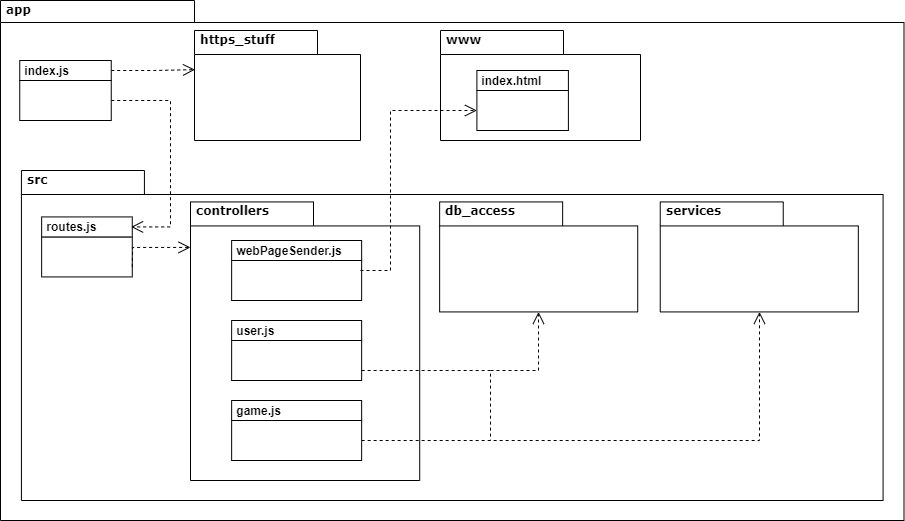
\includegraphics
	[width=1.2\linewidth]
	{package diagram - Server Side}
	\caption{package diagram dell'organizzazione server side.
		\newline
		Per applicare maggiore chiarezza, il formalismo del package diagram è stato violato e sono stati inseriti alcuni file, ma concettualmente il diagramma rappresenta comunque l'organizzazione e la dipendenza dei package e dei file rappresentati (i file rappresentati hanno estensione \texttt{js}, perché il progetto Nim Multiplayer è realizzato con la piattaforma Node e quindi è scritto in Javascript, ma a prescindere dal linguaggio usato, l'organizzazione di progetto deve essere questa).}
	\label{fig: package diagram - server side}
\end{figure}

\begin{enumerate}
\item
	Il file \texttt{index.js} è l'entry point dell'applicazione (il file eseguibile principale): connette l'applicazione al database; inizializza librerie e servizi dell'applicazione web; avvia il server.
\item
	Questo progetto adotta il pattern MVC nel web, per cui i controller agiscono tramite le rotte dell'applicazione, quindi il file \texttt{routes.js} definisce le funzionalità di sistema ed utilizza i controller per soddisfare le richieste.
\item
	Considerando quanto espresso fino ad ora, sono state individuate le responsabilità sottostanti, e ciascuna di esse è stata mappata da un corrispettivo controller rappresentato in figura \ref{fig: package diagram - server side}.
	\begin{itemize}
		\item
		Inviare la SPA verso il client che contatta il server
		\newline
		(\texttt{controllers/webPageSender.js}).
		\item
		Gestire il dominio dei dati utente, tramite chiamate Axios
		\newline
		(\texttt{controllers/user.js}).
		\item
		Gestire il dominio del gioco, tramite chiamate Axios e Socket.IO
		\newline
		(\texttt{controllers/game.js}).
	\end{itemize}
	(In figura \ref{fig: package diagram - server side} sono rappresentati tutti i controller di sistema.)
\item
	Infine, in figura \ref{fig: package diagram - server side} sono rappresentati i package sottostanti.
	\begin{itemize}
	\item
		\texttt{https\_stuff}: contiene il certificato e la chiave https.
	\item
		\texttt{db\_access}: considerando il pattern MVC, contiene gli elementi che rappresentano i model, cioè i file che accedono al database.
	\item
		\texttt{services}: contiene i file che forniscono ulteriori servizi, ad esempio: \texttt{services/user/passwordEncryption.js}.
	\end{itemize}
	Come già ribadito più volte, il sistema modella 2 domini distinti, gli utenti e il gioco, per cui \texttt{db\_access} e \texttt{services} contengono a loro volta i 2 sub-package \texttt{user} e \texttt{game} per migliorare l'organizzazione del codice.
\end{enumerate}

\paragraph{Accesso alla Persistenza: directory \texttt{db\_access} e directory \texttt{db\_access/models} \paragraphNewline}

\removeHorizontalSpaceSmall Un'importante scelta di design coinvolge la directory \texttt{app/src/db\_access} e la sua sub-directory \texttt{db\_access/models}. La directory \texttt{db\_access/models} deve contenere i modelli che rappresentano le entità salvate nel database, mentre la directory \texttt{db\_access} deve contenere gli oggetti che dispongono di metodi per manipolare tali entità ed operare sul database.
\newline
In questo modo, il codice risulta notevolmente leggibile e flessibile, ovvero le dipendenze della libreria utilizzata per interfacciarsi al database, sono totalmente incapsulate dentro i file di \texttt{db\_access}, per cui si può cambiare tecnologia di interfacciamento al database, semplicemente modificando i file di \texttt{db\_access} e di \texttt{db\_access/models}.
\newline
Un esempio di codice per comprendere questi vantaggi è riportato in \ref{persistenza: db_access - Codice}.

Questa organizzazione di codice appena descritta, è una sorta di pattern adapter\footnote{Adapter design pattern, descritto in GoF\citep{GoF}.}, in cui l'adaptee è la libreria scelta per interfacciarsi al database e gli adapter sono gli oggetti di \texttt{db\_access}.

Un altro esempio strutturalmente identico a questo tipo di pattern adapter, è osservabile nel file \texttt{app/src/services/user/passwordEncryption.js}, quest'ultimo adatta (seppur in maniera estremamente minimale) la libreria scelta per cifrare e decifrare la password nel database.

\newpage

\paragraph{Persistenza: Dati degli Utenti \paragraphNewline}

\removeHorizontalSpaceSmall Per memorizzare i dati degli utenti, è sufficiente disporre uno spazio di archiviazione che ammette solamente una tipologia di dato omogenea. I dati degli utenti memorizzati sono sempre gli stessi per ogni utente: l'identificativo (cioè l'username); la password; l'email (che è un secondo identificativo).

\paragraph{Persistenza: Stato delle Partite \paragraphNewline}

\removeHorizontalSpaceSmall Per memorizzare lo stato delle partite è assolutamente consigliato l'impiego di una tecnologia di persistenza NoSQL, perché il numero dei bastoncini e il numero di giocatori sono valori variabili per ogni partita (ma non solo, vi sono anche altri valori illustrati qui di seguito che sono variabili), pertanto NoSQL permette di gestire queste caratteristiche dinamiche con facilità.

Un dettaglio interessante inerente alla memorizzazione delle partite, è che indipendentemente dalla loro configurazione, il loro schema è sempre lo stesso, sia che una partita abbia modalità di vittoria Standard o Marienbad, sia che una partita abbia i turni in rotazione oppure chaos.

I dati memorizzati all'interno di uno schema di una partita sono riportati nel seguente elenco, e per ognuno di essi viene descritto come il loro valore influenza il comportamento di gioco.
\begin{itemize}
\item
	\texttt{sticks}: rappresenta i bastoncini, è un dato variabile per ogni partita, ed è rappresentato come una matrice, cioè un array di array in cui quest'ultimi sono le righe che contengono i valori dei bastoncini.
	\newline
	I valori dei bastoncini sono impostati inizialmente a false, e questo rappresenta lo stato di "bastoncino rimosso = false". Per gestire tutte le casistiche di configurazione di una partita, quando un bastoncino viene rimosso, nel valore del bastoncino viene inserito il nome del giocatore che lo ha rimosso. In questo modo, nelle partite Marienbad multiplayer, quando un giocatore viene eliminato, si possono facilmente ripristinare tutti i bastoncini rimossi dai giocatori presenti in gioco (come richiesto in \ref{requisiti funzionali}).
	\newline
	(Nel caso di una partita con modalità di vittoria Standard multiplayer, o nel caso di una partita 1 vs 1, sarebbe sufficiente inserire true come valore nei bastoncini rimossi, ma per semplicità si è scelto di adottare la soluzione appena descritta per soddisfare i vincoli di tutte le tipologie di partite.)
\item
	\texttt{standardVictory}: rappresenta la modalità di vittoria, è un valore booleano, \texttt{true} significa che la partita ha vittoria Standard, \texttt{false} significa che la partita ha vittoria Marienbad.
\item
	\texttt{turnRotation}: rappresenta la rotazione dei turni, è un valore booleano, \texttt{true} significa che i turni sono in rotazione, \texttt{false} significa che i turni sono chaos.
\item
	\texttt{activePlayer}: è una stringa che contiene l'username del giocatore di turno.
\item
	\texttt{players}: è un array con dimensione variabile che contiene gli username degli utenti in partita.
	\newline
	Il suo significato cambia in base alla modalità di rotazione dei turni.
	\begin{itemize}
	\item
		se \texttt{turnRotation} è uguale a \texttt{true}, allora i turni dei giocatori sono alternati per tutta la partita, seguendo l'ordine di \texttt{players}, generato casualmente ad inizio partita.
	\item
		se \texttt{turnRotation} è uguale a \texttt{false} (turni chaos), allora \texttt{players} contiene i giocatori che devono svolgere il turno. Quando un giocatore svolge il suo turno, viene inserito in \texttt{playersWithTurnDone}. Quando \texttt{players} è vuoto e \texttt{playersWithTurnDone} contiene tutti i giocatori, allora tutti i giocatori vengono rimossi da \texttt{playersWithTurnDone} per essere inseriti dentro \texttt{players}.
	\end{itemize}
\item
	\texttt{playersWithTurnDone}: è un array con dimensione variabile che contiene gli username degli utenti che hanno svolto il proprio turno.
	\newline
	Questo dato viene utilizzato solo nelle partite con turni chaos.
\item
	\texttt{eliminatedPlayers}: è un array con dimensione variabile che contiene gli username degli utenti eliminati dalla partita.
\item
	\texttt{disconnectedPlayers}: è un array con dimensione variabile che contiene gli username degli utenti disconnessi, e che devono essere eliminati dalla partita nel momento in cui si presenta il loro turno.
\end{itemize}

\subsubsection{Front-end vs Back-end}
\label{front-end vs back-end}

In tutte le applicazioni web, si deve cercare di spostare quanto più possibile l'application logic a client side, in modo da ridurre il carico di lavoro del server.

\paragraph{Rotte del Dominio dei Dati Utente \paragraphNewline}

\removeHorizontalSpaceSmall Per il motivo appena descritto, nella pagina di registrazione, è la SPA che deve avere la responsabilità di eseguire i controlli riguardo l'inserimento degli input field. In seguito, il server si deve occupare di verificare che: l'username e la mail non sono dati già registrati; l'username non supera una certa lunghezza, perché altrimenti questo causa problemi di renderizzazione dell'username durante il gioco (questo controllo è stato inserito a server side, perché è stato ritenuto più "sicuro" svolgerlo lì).

Allo stesso modo, nella pagina di login, è la SPA che deve avere la responsabilità di eseguire i controlli riguardo l'inserimento degli input field. In seguito, il server si deve occupare di svolgere i controlli sul database.

\paragraph{Rotta della Stanza di Gioco \paragraphNewline}

\removeHorizontalSpaceSmall Sempre per lo stesso motivo, nella pagina di gioco, è la SPA che deve avere la responsabilità di validare la mossa prima di inviarla al server. In seguito, il server si deve occupare di applicare la mossa alla partita, e gestire le disconnessioni dei giocatori in caso si verifichino.

\newpage
\section{Tecnologie}

L'applicazione è stata realizzata con il solution stack MEVN: MongoDB;
\newline
Express.js; Vue.js; Node.js.

All'inizio e durante lo svolgimento del progetto, si è considerato se utilizzare anche un game framework, come ad esempio Phaser, tuttavia questa opzione è stata scartata perché il funzionamento del gioco è estremamente semplice, e per modellarlo è stato sufficiente il solution stack proposto.

Inserire un game framework avrebbe forse reso l'applicazione più "pesante" senza trarre alcun significativo vantaggio, anche se, non conoscendo alcun game framework di Node, mi azzardo a supporre che forse avrebbe potuto rendere il codice del "game room" più modulare e meglio organizzato.

\subsection{Back-end}

\subsubsection{MongoDB}

Come già scritto nel design, la flessibilità di NoSQL e del formato documentale di MongoDB, hanno permesso di svolgere una significativa economia concettuale (le partite si modellano con un solo schema), la quale non sarebbe stata applicabile sfruttando il modello SQL relazionale.

Questo vantaggio è osservabile nello schema che rappresenta una partita: \texttt{app/src/db\_access/models/game.js}.

\subsubsection{Node.js}

Node è una piattaforma software che impiega un modello I/O non bloccante e ad eventi. Per questo, Node è una piattaforma dotata di elevata scalabilità, altamente indicata per \emph{data-intensive real-time} (DIRT) application (tra cui videogiochi online) che gestiscono un elevato numero di connessioni simultanee.

Node possiede il più grande ecosistema di librerie open source al mondo, e in questo progetto sono state utilizzate le seguenti.
\begin{itemize}
\item
	\texttt{mongoose} per interfacciarsi al database.
\item
	\texttt{express} per usare il framework Express.js.
\item
	\texttt{cors} per impostare le politiche CORS.
\item
	\texttt{express-session} per gestire la sessione (cookie) di Express.js.
\item
	\texttt{socket.io} per utilizzare la libreria Socket.IO a server side.
\item
	\texttt{bcrypt} per cifrare le password nel database.
\end{itemize}

\subsubsection{Express.js}

Express è un framework server side per applicazioni web, minimale e flessibile. Facilita l'implementazione di API REST in Node.

\newpage

\subsection{Front-end}

\subsubsection{Vue.js}

Vue permette di sviluppare SPA reattive sfruttando il dual-binding tra modello dati e vista. Vue implementa il paradigma \emph{Model-View-ViewModel} (MVVM), in particolare si focalizza sul ViewModel layer che connette la View con il Model attraverso un two way data binding. Vue rende possibile implementare un'applicazione ragionando in termini di dati, variabili e oggetti, astraendosi rispetto al DOM della pagina, seppur usando comunque le viste HTML.

\subsubsection{Bootstrap, CSS e SCSS}

In questo progetto è stato utilizzato SCSS, ovvero un'estensione del linguaggio CSS, eseguito da preprocessor (o transpiler) SASS.

Il linguaggio SCSS viene accompagnato dal framework Bootstrap, il quale offre responsive design e layout liquido.

Bootstrap fornisce davvero tantissime funzionalità e ciò lo rende un framework "pesante". In questo progetto si è sperimentato un'alternativa per alleggerire Bootstrap, ovvero invece di importare l'intera libreria a client-side tramite content delivery network (CDN), Bootstrap è stato inserito a server side tramite il suo corrispondente node module in versione SCSS. Dopodiché nel file di presentazione SCSS (\texttt{app/www/public/scss/style.scss}) sono stati importati ed utilizzati solo gli elementi di Bootstrap necessari per lo stile del progetto, e infine il file SCSS è stato tradotto nel file CSS (\texttt{app/www/public/css/style.css}) da inviare al client.

Innestare Bootstrap nel SCSS in questo modo, comporta alcuni trade-off rispetto ad importarlo tramite CDN.
\begin{itemize}
\item
	Il server di Nim Multiplayer invia un file CSS più grande rispetto al file che dovrebbe inviare tramite la soluzione CDN.
	
	Il file CSS inviato dal server di Nim Multiplayer contiene: gli elementi di Bootstrap inclusi nel file SCSS e gli elementi specifici di progetto.
	
	Nella soluzione CDN: gli elementi di Bootstrap sono reperibili tutti via CDN e il file CSS inviato dal server di Nim Multiplayer contiene solamente gli elementi specifici di progetto.
	
	Il file CSS inviato dal server di Nim Multiplayer, è più piccolo della libreria Bootstrap reperibile tramite CDN.
	
	Quindi in questo modo Bootstrap è più "leggero" a client side.
\item
	Nel file SCSS è possibile attribuire ai type selector ({\texttt{body}, \texttt{section}, ...}) direttamente le classi degli elementi di Bootstrap (il type selector esegue la \texttt{@extend} delle classi di Bootstrap), in questo modo si evita, in maniera minima, ma rilevante, di inserire le classi di Bootstrap nella parte strutturale di HTML.
\end{itemize}

\subsection{Back-end e Front-end}

\subsubsection{Socket.IO}

Per le comunicazioni real-time si è scelto di impiegare la libreria Socket.IO.

L'unica feature utilizzata è quella più semplice, e coinvolge solamente il concetto di evento emesso ed ascoltato da un sottoinsieme di client.

Socket.IO fornisce anche il concetto di room (server side), tuttavia non è stato utilizzato questo tipo di astrazione, perché semplicemente non si ha avuto l'esigenza di farlo, ovvero una partita può essere modellata semplicemente come un singolo evento, in cui giunge la mossa svolta dal giocatore attivo oppure la disconnessione di un giocatore.

\newpage
\section{Codice}

\subsection{Front-end}

\subsubsection{Organizzazione (Design) del Codice SCSS}

Il package \texttt{public/scss} rispecchia la struttura del package \texttt{public/js} illustrata nella sezione \ref{design architettura - front-end}. Il package \texttt{public/scss} contiene gli elementi sottostanti.
\begin{enumerate}
\item
	 Il file \texttt{style.scss} che viene eseguito con preprocessor SASS per generare il suo file corrispettivo: \texttt{public/css/style.css}. Quest'ultimo (come già spiegato) è il layer di presentazione da importare in \texttt{www/index.html}.
	 \newline
	 Il file \texttt{style.scss} deve contenere solo i selettori SCSS di elementi e classi utilizzate fra due o più rotte.
\item
	Il package \texttt{routes}: ogni file contenuto in questo package contiene i selettori SCSS di elementi contenuti in una rotta dell'applicazione; per ogni file contenuto in \texttt{public/js/routes} può esistere 1 o 0 file di presentazione collocato in questo package. 
\item
	Il package \texttt{elements}: ogni file contenuto in questo package contiene i selettori SCSS di una porzione di html incapsulata e riutilizzata fra le rotte dell'applicazione; per ogni file contenuto in \texttt{public/js/elements} può esistere 1 o 0 file di presentazione collocato in questo package. 
\end{enumerate}

\subsubsection{Il "Pattern": \texttt{errorMessage}}

\texttt{errorMessage} è un "pattern" che è stato improvvisato ed inserito in questo progetto per migliorare la leggibilità e la qualità del codice. "Pattern" è posto tra virgolette perché chiaramente non è pattern vero e proprio, e non è neppure una porzione di codice modularizzata, perché purtroppo non è stato trovato alcun modo per farlo. Tuttavia è una forma di codice che è stata ripetuta in più punti a client side, perché si ritiene che sia particolarmente efficace per rendere maggiormente comprensibile il codice.

Molti Vue component (contenuti nei package \texttt{js/routes} o in \texttt{js/elements}) contengono nel proprio insieme di dati, il dato \texttt{errorMessage}. Come suggerisce il nome, questo dato rappresenta il messaggio di errore comunicato all'utente che sta interagendo con l'applicazione. Questo dato viene utilizzato da alcune operazioni come una sorta di stato, per capire se continuare a procedere con l'esecuzione in corso: se \texttt{errorMessage} possiede contenuto, allora si è già verificato un errore e l'operazione non deve procedere, oppure l'operazione deve continuare a verificare se ci sono altri errori da comunicare all'utente, concatenandoli al contenuto di \texttt{errorMessage} generato precedentemente.

Un'altra forma di codice ritenuta molto comprensibile e che spesso accompagna \texttt{errorMessage}, sono le funzioni \texttt{gatherClientSideErrorsFrom(vueComponent)} e \texttt{gatherServerSideErrorsFrom(response)}, i quali si occupano entrambi di "raccogliere" gli errori, elaborare un messaggio di errore, e restituirlo come valore di ritorno con cui impostare il valore di \texttt{errorMessage}.
\newline
In alcuni punti si potrebbero avere alcune varianti di queste funzioni, ma l'idea di fondo è piuttosto intuibile e rimane sempre la stessa.

Nel codice sottostante, ecco un esempio di utilizzo di questo "pattern", nel Vue component che rappresenta la pagina di registrazione di un nuovo utente: \texttt{app/www/public/js/routes/user/register.js}.
\begin{lstlisting}
...
	<p v-html="errorMessage" class="error-message"></p>
...
data() {
	return {
		...
		errorMessage: '',
	}
},
...
methods: {
	register: function(event) {
		event.preventDefault()
		this.errorMessage = gatherClientSideErrorsFrom(this)
		if (this.errorMessage === '') {
			const credential = {
				username: this.username,
				email: this.email,
				password: this.password
			}
			axios.post(serverAddress + 'register', credential)
			.then((response) => {
				this.errorMessage = gatherServerSideErrorsFrom(response)
				if (this.errorMessage === '') {
					registrationSuccessful(this)
				}
			})
			.catch((error) => { this.errorMessage = error })
		}
		
		function gatherClientSideErrorsFrom(vueComponent) { ... }
		
		function gatherServerSideErrorsFrom(response) { ... }
	}
...
\end{lstlisting}

\newpage

\subsubsection{Elementi di Design aggiunti durante l'Implementazione}

Il package \texttt{public/js/routes/utilities} contiene 2 file di utility.
\begin{itemize}
\item
	\texttt{two-page-routing.js} gestisce la navigazione rappresentata dalla storyboard in figura \ref{fig:storyboard - user session}. Questa utility è stata modularizzata in questo modo, perché l'utente può svolgere quella storyboard anche partendo dalla rotta rappresentata dal file \texttt{public/js/routes/create-game-room.js}, di conseguenza sfruttando \texttt{two-page-routing.js} non si ha codice duplicato.
\item
	\texttt{session-utilities.js} racchiude varie utility inerenti alla sessione di login dell'utente, applicabili ad un'istanza di Vue. Anche questa scelta di design serve ad applicare il principio DRY, oltre ad incapsulare un insieme di responsabilità ben precise.
\end{itemize}

\subsection{Back-end}

\subsubsection{Accesso alla Persistenza: directory \texttt{db\_access} e directory \texttt{db\_access/models}}
\label{persistenza: db_access - Codice}

Nel file \texttt{controller/user.js} si utilizza: \texttt{db\_access/user.js}.

\begin{lstlisting}
const usersCollection = require('../db_access/user')

...

exports.logIn = function(req, res) {
	...
	usersCollection.findUserByUsername(username)
	...
\end{lstlisting}

\removeHorizontalSpaceBig Mentre nel file \texttt{db\_access/user.js} si utilizzano: la libreria \texttt{mongoose} per interfacciarsi al database e il suo modello \texttt{db\_access/models/user.js}.

\begin{lstlisting}
const mongoose = require('mongoose')
const UserModel = require('./models/user')
const User = UserModel(mongoose)

...

exports.findUserByUsername = function(username) {
	return User.findById(username).lean()
}
...
\end{lstlisting}

\newpage

\subsubsection{Un Raro Errore di Interazione}

Se il giocatore di turno (giocatore attivo) invia la mossa nell'esatto momento in cui un altro giocatore si disconnette, entrambi gli eventi potrebbero modificare nello stesso momento l'istanza di gioco salvata nel database, causando comportamenti imprevedibili. È un problema molto raro, ma può comunque verificarsi. Ad ogni modo, esso è facilmente risolvibile inserendo un monitor per regolare l'accesso al database di quella specifica partita, tra i due handler degli eventi.

Non ho implementato questo monitor, sia per mancanza di tempo, sia perché comunque è un problema molto raro, e anche perché non sapevo esattamente come testarlo, poiché dato che è letteralmente impossibile inviare contemporaneamente una mossa e una disconnessione "manualmente" utilizzando due schede diverse del browser, avrei dovuto utilizzare un sistema di test più complesso e non ne sarebbe valsa la pena in termini di tempo speso per realizzarlo e guadagno effettivo nel testare il caso in questione.

\newpage

\section{Test}

\subsection{Acceptance Test}

Il design riportato in \ref{design delle interfacce utente} può essere considerato una sorta di acceptance test.

\subsection{Acceptance e Functional Test degli Errori Utente}

In questa sezione vengono descritti i test riguardo l'utilizzo di ogni pagina con l'obiettivo di generare tutti gli errori possibili (functional test degli errori utente), e verificare la correttezza del messaggio di errore generato, valutandone la qualità in termini di comunicazione con l'utente (acceptance test degli errori utente).

\subsubsection{Network Error}

Un test che può essere eseguito in molteplici punti dell'applicazione, riguarda la visualizzazione dell'assenza di connessione da parte del client o del server durante l'esecuzione di una Axios request, e si può svolgere nel seguente modo.

Prima di fare eseguire all'applicazione una request tramite Axios, si deve arrestare l'esecuzione del server, dopodiché si fa eseguire all'applicazione tale Axios request. In questo modo, dopo qualche secondo Axios genera (a client side) una exception avente come messaggio di errore "Error: Network Error", visibile dall'utente nel HTML paragraph dedicato agli errori (\texttt{errorMessage}).

Dopo questa constatazione, se la request inviata non richiede una situazione particolare per avere successo, si può avviare il server e (senza refreshare la pagina) rieseguire la Axios request fallita precedentemente, la quale questa volta non genera più il Network Error, perché ovviamente ora il server può rispondere.

Si riporta ora un'osservazione riguardo le exception generate da Axios e un test "irrilevante" che è stato eseguito giusto per curiosità. Axios genera le exception basandosi sulla response ricevuta (o non ricevuta, nel caso del Network Error), ad esempio, se Axios riceve HTTP status code 500, allora genera una exception avente come messaggio di errore "Error: Request failed with status code 500". Il test "irrilevante" riguarda proprio questa exception. Viene definito "irrilevante" perché in condizioni normali non dovrebbe mai verificarsi, ad ogni modo, il test eseguito consisteva nel modificare il codice a server side, in modo che il server rispondesse con il codice di errore HTTP 500, ed il client visualizzava l'errore in pagina.

In conclusione, si vuole affermare che, il test "Network Error" equivale al verificare la visualizzazione di un qualsiasi altro errore generato da Axios (il codice che gestisce la visualizzazione del Network Error è lo stesso utilizzato per gestire tutte le eccezioni di Axios), pertanto l'utente è sempre più o meno consapevole della situazione in cui si trova.

\newpage

\subsubsection{Registration Page}

Test da eseguire per innescare tutti gli errori del client side.
\begin{itemize}
\item
	Lasciare tutti gli input field vuoti e cliccare il bottone \textbf{Sign up}, dopodiché leggere il messaggio di errore generato, e inserire i valori negli input field in modo da verificare tutte le combinazioni del messaggio di errore.
\end{itemize}

\removeHorizontalSpaceBig Test da eseguire per innescare tutti gli errori del server side.
\begin{itemize}
\item
	Inserire un username già esistente nel database.
\item
	Inserire una email già esistente nel database.
\item
	Inserire un username troppo lungo.
\item
	Eseguire il login e visitare questa pagina inserendo nella barra degli indirizzi il suo path (\texttt{/register}), a questo punto si verrà reindirizzati alla home page.
\end{itemize}

\subsubsection{Login Page}

Test da eseguire per innescare tutti gli errori del client side.
\begin{itemize}
\item
	Lasciare entrambi o 1 degli input field vuoti e cliccare il bottone \textbf{Sign in}.
\end{itemize}

\removeHorizontalSpaceBig Test da eseguire per innescare tutti gli errori del server side.
\begin{itemize}
\item
	Inserire username e password non esistenti, oppure username e password sbagliati.
\item
	Eseguire il login e visitare questa pagina inserendo nella barra degli indirizzi il suo path (\texttt{/login}), a questo punto si verrà reindirizzati alla home page.
\end{itemize}

\subsubsection{Account Page}

Test da eseguire per innescare tutti gli errori del server side.
\begin{itemize}
\item
	Senza eseguire il login, visitare questa pagina inserendo nella barra degli indirizzi il suo path (\texttt{/account}), a questo punto si verrà reindirizzati alla home page.
\item
	Eseguire il login, e aprire questa pagina in 2 schede dello stesso browser, dopodiché effettuare il log out (o cancellare definitivamente l'account) in una pagina e poi cancellare definitivamente l'account (o effettuare il log out) nell'altra.
\end{itemize}

\newpage

\subsubsection{Create Game Room Page}

Test da eseguire per innescare tutti gli errori del server side.
\begin{itemize}
\item
	Senza eseguire il login, cliccare sul bottone \textbf{CREATE GAME ROOM}.
\end{itemize}

\subsubsection{Game Room Page - Invite other Players!}

Test da eseguire per innescare tutti gli errori del client side.
\begin{itemize}
\item
	Cliccare sul bottone \textbf{Start Game!} mentre nel game room c'è 1 utente.
\item
	Cliccare sul bottone \textbf{Start Game!} mentre nel game room c'è un numero di utenti superiore al numero massimo consentito.
\end{itemize}

\removeHorizontalSpaceBig Test da eseguire per innescare tutti gli errori del server side.
\begin{itemize}
\item
	Senza eseguire il login, visitare un game room in attesa di giocatori.
\item
	Senza eseguire il login (oppure anche dopo aver eseguito il login), visitare la pagina di una partita non esistente (può avere un semplice \_id inventato, ad esempio "abc123", oppure può avere un \_id appartenente a MongoDB, il messaggio di errore generato è lo stesso in entrambi i casi)
\end{itemize}

\subsubsection{Game Room Page - Time to play the game!}

Test da eseguire per innescare tutti gli errori del client side.
\begin{itemize}
\item
	Durante la partita, rimuovere 0 bastoncini.
\item
	Durante la partita, selezionare e rimuovere bastoncini che non sono nella stessa riga.
\item
	Durante la partita, selezionare e rimuovere bastoncini nella stessa riga, ma non adiacenti.
\end{itemize}

\removeHorizontalSpaceBig Test da eseguire per innescare tutti gli errori del server side.
\begin{itemize}
\item
	Eseguire il login, e visitare una pagina di un gioco già iniziato.
\end{itemize}

\subsubsection{Game End Page}

Test da eseguire per innescare tutti gli errori del server side.
\begin{itemize}
\item
	Senza inviare parametri via POST, visitare questa pagina inserendo nella barra degli indirizzi il suo path (\texttt{/game-end}), a questo punto si verrà reindirizzati alla home page.
\end{itemize}

\newpage

\subsection{Functional Test del Gioco}

Test da eseguire per verificare il corretto funzionamento del gioco, in particolare per accertarsi che i requisiti siano soddisfatti.
\newline
(Lo svolgimento delle partite 1 vs 1, aventi qualsiasi configurazione, è considerato triviale e quindi non viene testato, anche perché il sottoinsieme di questo tipo di partite, viene verificato nei seguenti test riguardo le partite multiplayer.)
\begin{itemize}
\item
	Creare e giocare 2 partite simultaneamente (possono avere gli stessi utenti oppure utenti diversi).
\item
	Controllare lo svolgimento dei turni, sia con vittoria Standard, sia con vittoria Marienbad.
	\begin{itemize}
	\item
		I turni in rotazione sono osservabili dall'interfaccia di gioco.
	\item
		I turni chaos, per testarli è consigliato svolgere una partita 1 vs 1 oppure svolgere una partita multiplayer con 3 giocatori, e notare che, prima o poi (in modo totalmente non deterministico), un giocatore invece di svolgere 1 turno alternandosi con gli altri giocatori, svolgerà (al massimo) 2 turni consecutivi.
	\end{itemize}
\item
	Verificare lo svolgimento di una partita multiplayer senza disconnessioni. Si ritiene che una partita con 4 giocatori sia ragionevolmente complessa.
	\begin{itemize}
	\item
		Una partita con turni in rotazione e vittoria Standard.
	\item
		Una partita con turni in rotazione e vittoria Marienbad.
	\item
		Una partita con turni chaos e vittoria Standard.
	\item
		Una partita con turni chaos e vittoria Marienbad.
	\end{itemize}
\end{itemize}

\subsubsection{Gestione delle Disconnessioni}

Eseguire i seguenti scenari per osservare il comportamento corretto della gestione delle disconnessioni. Si ricorda che le disconnessioni vengono gestite quando si presenta il turno del giocatore disconnesso.
\newline
Anche in questo caso, si considera una partita con 4 giocatori, con i \ul{turni in rotazione}, e gli scenari sottostanti devono essere svolti sia con vittoria Standard, sia con vittoria Marienbad.
\begin{itemize}
\item
	Disconnettere il giocatore di turno successivo rispetto al giocatore attivo (1 disconnessione), ed eseguire la mossa del giocatore attivo.
	
	Applicare questo scenario in 2 casi.
	\begin{enumerate}
		\item
		Dopo la disconnessione, deve rimanere in gioco un solo giocatore, e quindi vince.
		\item
		Dopo la disconnessione, devono rimanere in gioco 2 o più giocatori, e continuare a giocare la partita fino alla fine.
	\end{enumerate}
\item
	Disconnettere i 2 giocatori di turno successivo rispetto al giocatore attivo (2 disconnessioni consecutive), ed eseguire la mossa del giocatore attivo.
	
	Applicare questo scenario in 2 casi.
	\begin{enumerate}
		\item
		Dopo le 2 disconnessioni, deve rimanere in gioco un solo giocatore, e quindi vince.
		\item
		Dopo le 2 disconnessioni, devono rimanere in gioco 2 o più giocatori, e continuare a giocare la partita fino alla fine.
	\end{enumerate}
\item
	Disconnettere il giocatore di turno (giocatore attivo).
	
	Applicare questo scenario in 2 casi.
	\begin{enumerate}
		\item
		Dopo la disconnessione, deve rimanere in gioco un solo giocatore, e quindi vince.
		\item
		Dopo la disconnessione, devono rimanere in gioco 2 o più giocatori, e continuare a giocare la partita fino alla fine.
	\end{enumerate}
\item
	Disconnettere il giocatore di turno successivo rispetto al giocatore attivo, e poi disconnettere il giocatore attivo, causando 2 disconnessioni consecutive.
	
	Applicare questo scenario in 2 casi.
	\begin{enumerate}
	\item
		Dopo le 2 disconnessioni, deve rimanere in gioco un solo giocatore, e quindi vince.
	\item
		Dopo le 2 disconnessioni, devono rimanere in gioco 2 o più giocatori, e continuare a giocare la partita fino alla fine.
	\end{enumerate}
\item
	Disconnettere i 2 giocatori di turno successivo rispetto al giocatore attivo, e poi disconnettere il giocatore attivo, causando 3 disconnessioni consecutive.
	
	Applicare questo scenario in 2 casi.
	\begin{enumerate}
		\item
		Dopo le 3 disconnessioni, deve rimanere in gioco un solo giocatore, e quindi vince.
		\item
		(Questo è l'unico caso in cui è necessaria una partita con 5 giocatori.) Dopo le 3 disconnessioni, devono rimanere in gioco 2 o più giocatori, e continuare a giocare la partita fino alla fine.
	\end{enumerate}
\end{itemize}
	
\removeHorizontalSpaceBig Eseguire questi scenari in una partita (sia con vittoria Standard, sia con vittoria Marienbad) con i \ul{turni chaos}, è piuttosto difficile perché la rotazione dei turni è casuale (anche se, in una situazione specifica si può prevedere quale sarà il giocatore attivo successivo, cioè si consideri il caso in cui ci sono 4 giocatori in partita e 2 di essi hanno già svolto il turno, allora si conosce il giocatore attivo ed il prossimo giocatore attivo). Ad ogni modo sono state eseguite svariate prove con i \ul{turni chaos} e sembra funzionare tutto a dovere.

\newpage
\section{Deployment}

Per installare ed eseguire l'applicazione si devono svolgere le seguenti istruzioni.
\begin{enumerate}
\item
	Installare \texttt{MongoDB}. Creare il database \texttt{nim\_multiplayer} e le collezioni \texttt{users} e \texttt{games}. Nella collezione \texttt{users} si devono impostare \texttt{username} e \texttt{mail} come identificativi primari.
\item
	Installare \texttt{Node.js} e \texttt{git}.
\item
	Clonare il repository:
	
	\texttt{git clone https://github.com/deividvd/Nim-Multiplayer/}
\item
	Tramite la command line, posizionarsi all'interno di \texttt{Nim-Multiplayer/app/}, e risolvere le dipendenze di \texttt{Node.js}:
	
	\texttt{npm install}
\item
	Eseguire l'applicazione:
	
	\texttt{node index.js}
\item
	Utilizzare l'applicazione tramite un browser all'indirizzo (la connessione sarà non sicura perché il certificato https è auto firmato):
	
	\texttt{https://localhost:3000}
\end{enumerate}

\newpage

\section{Conclusioni}

Mi ritengo soddisfatto dell'applicazione realizzata, ho implementato un gioco vero e proprio, seppur semplice, inoltre penso che il codice è scritto e organizzato in modo comprensibile ed efficiente per garantirne il riuso e la modifica, nonostante fosse la mia prima esperienza di programmazione full stack con Javascript.

Per migliorare ulteriormente il gioco, può essere aggiunto un limite di tempo per svolgere la mossa. Eventualmente si può aggiungere anche una chat dentro le stanze di gioco, tuttavia questa chat non è particolarmente necessaria perché ovviamente si presume che i giocatori si conoscano e quindi se lo desiderano possono usufruire di chat di terze parti come ad esempio Discord.

\newpage

\bibliographystyle{plain}
\bibliography{references}

\end{document}